\chapter{Model of distribution grids}
\label{ch:distrib}
\minitoc

It has long been acknowledged that load models play have a critical influence on the results of dynamic simulations, especially on voltage stability~\cite{kundur}. Most utilities however use relatively (e.g. compared to generators) simple load models due to the difficulty to gather data on the loads connected to the distribution grid and their variable nature\footnote{Both the total amount of load and shares of different types of loads (heaters, motors, lamps, etc.) vary with the time of day and the season.}. The most commonly used model is the ZIP load model (aggregation of a constant impedance, a constant current and a constant power load) and its derivatives~\cite{IndustryLoadModel}.

The massive installation of distributed renewable energy sources (mostly wind and solar) in distribution grids challenges those load models. In particular interest in this thesis is the tendency of distributed generators to disconnect during wide-area disturbances. These disconnection had a high impact in historical blackouts. For example, the frequency collapse of Italy in 2003 was partly caused by the unexpected disconnection of 3400~MW of distributed generators while the frequency was still above 49~Hz~\cite[p115]{Italy2003}. On the other hand, there are perspectives regarding the provision of ancillary services by distributed generators. Better modelling of those so-called active distribution networks (ADNs) is thus needed.

One way to accurately model the interactions between the transmission and distribution sides of a grid is to perform simulations on complete a transmission and distribution network as in~\cite{FullTDexample}\footnote{To limit the size of the studied system, it is of course necessary to only consider the medium voltage level of the distribution grids, not the low voltage level.}. However, this approach cannot be used in this thesis due to the high computational power requirements of probabilistic dynamic security assessment. Outside the scope of this thesis, this approach also has issues of confidentiality and data handling.

% Co-simulation of T\&D (gridlabd?)

Reduced-order load models are thus necessary. Section~\ref{sec:dynLoadModel} thus reviews load models used in the literature%, and section~\ref{sec:dynLoadModelParam} discussed how to estimate the parameters of these load models.
and section~\ref{sec:loadPerspectives} discusses perspectives.

\section{Passive load models}
\label{sec:dynLoadModel}

Load models have seen renewed interest in the past decade due post-mortem reproduction of some blackouts being impossible with simple ZIP models~\cite[p11-12]{CIGREloadModels}. It was shown necessary to include at least a simple model of induction machines as in Figure~\ref{fig:motorLoad}. The model of the induction machine can be either static (i.e. only include algebraic equations, so consider the slip \(s\) to be constant) or dynamic (i.e. differential-algebraic equations, so the slip varies with time as a function of the balance between the electromagnetic and load torques). More complex load models such as the WECC composite load model (CLM) have also been developed. The CLM is shown in Figure~\ref{fig:WECC-CLM}. It consists in an on-load tap changer (OLTC), and equivalent feeder impedance, four different types of dynamic induction motor models, and electronic and a static (i.e. ZIP) load. It is being implemented in several time-domain simulators~\cite{NERCloadModelTF}. Various models whose complexity is between the ZIP and CLM models have also been developed and are reviewed by the CIGRE~\cite{CIGREloadModels} and NERC~\cite{NERCloadModelTF} task forces on load modelling.

\begin{figure}[t]
    \centering
    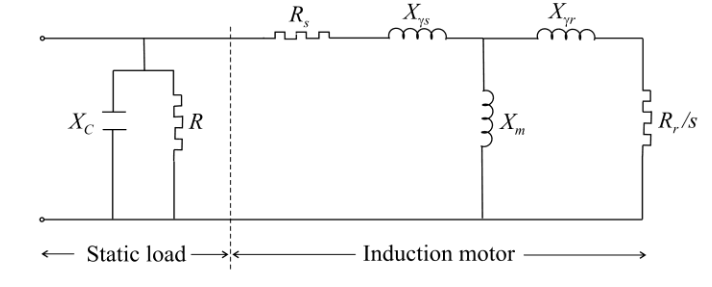
\includegraphics[width=0.6\linewidth]{Figs/MotorLoad.png}
    \caption{Constant impedance load in parallel with an induction motor~\cite{CIGREloadModels}}
    \label{fig:motorLoad}
\end{figure}

\begin{figure}[t]
    \centering
    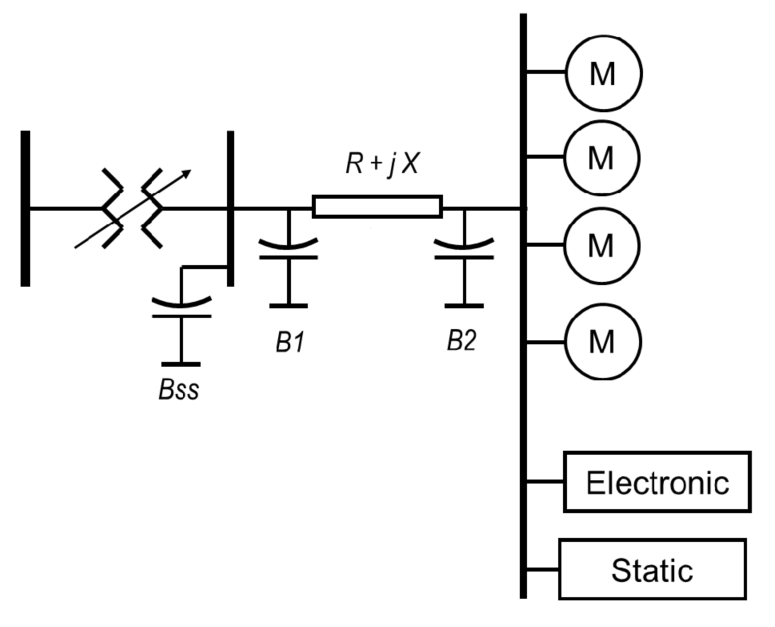
\includegraphics[width=0.5\linewidth]{Figs/WECC-composite-load-model.png}
    \caption{WECC composite load model~\cite{NERCloadModelTF}}
    \label{fig:WECC-CLM}
\end{figure}

The models presented above however do not consider distributed energy sources. The simplest solution to this is to add one (or several) generic model(s) of renewable sources to the load model. However, estimating the parameters that give the most accurate representation of the system might be difficult, especially since TSOs have little experience with ADNs compared to ZIP and motor load models. So, four main types of methods were developed in the literature to build ADNs models. They are listed below~\cite{ADNreview2013}.

\begin{itemize}
    \item Linear-based approaches: in these methods, the model of the full distribution network is first linearised. Then, different approaches (e.g. Hankel-norm approximation, modal approach, Krylov methods, etc.) allow to reduce the order of the linearised system. A theoretical bound on the error made by using the reduced-order model can be derived depending on the method used. These methods are however accurate only around a given operating point and are thus not appropriate to study large disturbances. These methods were originally developed to make reduced-order equivalents of neighbouring transmission systems. Indeed, TSOs mostly study the impact of disturbances originating in their own system. For moderately large disturbances, neighbouring TSOs are weakly affected, so a linearisation-based approach makes sense. Distribution systems however are much more dependant on their associated transmission system.
    \item Coherency-based approaches: synchronous generators that tend to swing together are grouped into an equivalent machine. The network around those machines is then also reduced. Like linear-based approaches, these methods were developed to model neighbour transmission systems. They are often not applicable to distribution systems as synchronous generators are rarely used there.
    \item Black-box approaches: in these methods, the model of a distribution system is an artificial neural network (ANN) that is trained to match the behaviour of the actual distribution system. These methods are quite popular since they do not require any information on the structure and components of the distribution grid. ANNs are thus most often matched to measurements of the behaviour of the distribution grid (often PMU measurements made at the point of common coupling (PCC) between the transmission and distribution grids). It is also possible to train ANNs from simulations of the distribution grid, but grey-box approaches (described below) are often preferred when one has enough information on the distribution grid to simulate it. The main limitation of measurement-based approaches (and by extension black-box approaches) is that large disturbances are rare. It is possible to intentionally introduce disturbances to generate more data but those disturbances are usually kept small for obvious reasons (usually tap changes or capacitor switching). Training ANNs for those disturbances is thus often impossible.
    \item Grey-box approaches: grey-box approaches are similar to black-box approaches except that the model used is a physical model instead of an ANN. The model usually has at most a few buses and should have a similar structure than the real grid\footnote{Taking the example shown in Figure~\ref{fig:greyBox}, if switches a and b are closed, and switch c is open, they grey-box model becomes two feeders in parallel. One feeder could represent a classical distribution system. The second, a large distribution-connected plant (with stricter connection requirements).}. The advantage is thus that results are more comprehensive, but it is necessary to known  the structure of the distribution grid. An example of grey-box model is shown in Figure~\ref{fig:greyBox}. Like black-box approaches, the parameters of the model are fitted to match the behaviour of the full model (e.g. in the least square sense). As it is not feasible to write the analytical formulation of the objective function (i.e. difference between behaviour of the grey-box and the real system), derivative-free optimisation methods (e.g. genetic algorithms, particle swarm optimisation) have to be used. The behaviour of the real system for a given operating point and disturbance can be obtained either from measurements or from simulations. As previously explained, only the simulation-based approach is appropriate when studying large disturbances\footnote{When available, measurements should still be used to validate the equivalent and/or the full distribution model.}.
\end{itemize}

\begin{figure}
    \centering
    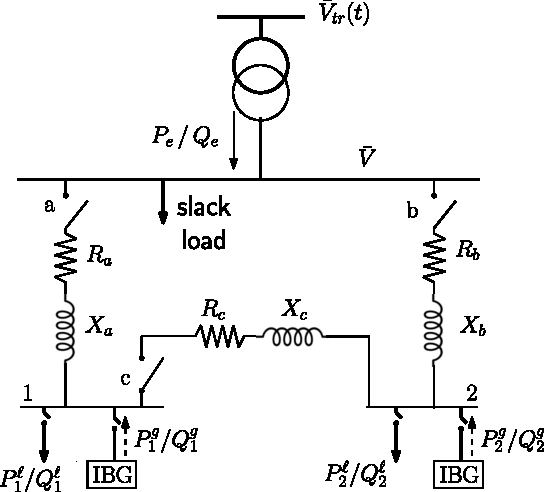
\includegraphics[width=0.6\linewidth]{Figs/GreyBoxEquivalent.pdf}
    \caption{Possible grey-box equivalent topologies. Multiple topologies can be created from this scheme by changing the status of the switches~\cite{ChaspierreThesis}. IBG = Inverter-based generation}
    \label{fig:greyBox}
\end{figure}


As discussed above, only (simulation-based) grey-box approaches are suitable to study large disturbances. This is thus the type of approach chosen in this thesis. Most recent development on grey-box approaches have been made in the thesis of Gilles Chaspierre~\cite{ChaspierreThesis, ChaspierrePaper}. His approach is thus used as a reference in this thesis. He also proposed a methodology to share the grey-box development between the TSO and DSOs to avoid confidentiality issues, and he discussed how to efficiently update the equivalent with varying operating conditions. Interestingly, he also proposed a control algorithm for a battery storage to be installed at the PCC to compensate for errors between the grey-box and the real system. Those elements are however not discussed further here.


\section{Perspectives}
\label{sec:loadPerspectives}

The results in~\cite{ChaspierreThesis} were very satisfactory, so relatively little improvements can be performed\footnote{A more detailed discussion of potential improvement is done in section 7.2 of~\cite{ChaspierreThesis}.}. Two main paths can be considered in this thesis. The first is the validation of grey-box models in large-scale studies. Indeed, in the literature, ADN equivalents (including grey-boxes, black-boxes, etc.) are validated in studies were only one distribution system is replaced by an equivalent (the others are simply considered to always behave as simple load models). In this thesis, studies will be performed by replacing all loads by equivalents. Additionally, as I study cascading outages, the models will be further challenged.

Another path to consider is the handling of model uncertainties. In~\cite{ChaspierreThesis}, the complete model of the distribution system is simulated with random sets of parameters (e.g. parameters of the control loops of distributed generation, share of renewables, etc.) to account for uncertainties. From these simulations, one deduces the average (i.e. statistical expected) behaviour of the system as well its standard deviation. This is illustrated in the example in Figure~\ref{fig:greyBoxUncertainty}. The grey-box is then fitting to the average, and the objective function is a least square error weighted by the standard deviation for each point in time. In the rest of the literature, uncertainties are not considered (except measurement errors in measurement-based approaches). In this thesis, I might try to determine if using a single equivalent is appropriate, or if using multiple equivalents associated with different realisations of the uncertainties is necessary. Also, methods to propagate the uncertainties from the full model to the equivalent might be considered. % Correlation between uncertainties of different distribution grids (e.g. LVRT of a given manufacturer)

% "Probabilistic load model": transfer the uncertainty in parameters of full model into the reduced one. And/or sensitivity studies.

\begin{figure}
    \centering
    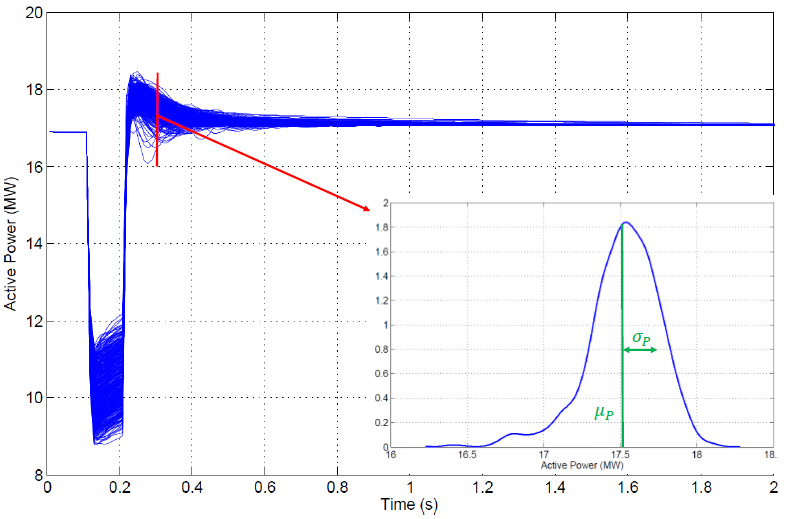
\includegraphics[width=0.6\linewidth]{Figs/GreyBoxUncertainty.png}
    \caption{Average \(\mu_P\) and standard deviation \(\sigma_P\) of the active power consumption of a distribution grid following a disturbance at \(t=\)0.3~s~\cite[p58]{ChaspierreThesis}}
    \label{fig:greyBoxUncertainty}
\end{figure}


Finally, as this thesis is made in the framework of the CYPRESS project (presented in appendix~\ref{ch:CYPRESS}), the possibility to include cyber elements in the equivalents will be studied.

\TODO{Fig of equivalent with average parameters vs. correct ones (in draft of ISGT paper), not fully accurate but already way better than simple load model}

\TODO{(fig 4 of CIGRE paper shows it would be best to cluster, but does not work for multiple disturbances)}


% Assume already have the appropriate load model for each moment of year -> do not include in computing time for DPSA